\documentclass[12pt,letterpaper]{article}

%Note to Self:
%When Decommission? - after two months of feeling useless or right away?

\usepackage[utf8]{inputenc}
\usepackage[letterpaper,margin=1in]{geometry}
\usepackage{caption} % for table captions

\usepackage{amsmath} % for multi-line equations and piecewises
\usepackage{indentfirst} % to indent after a section
\usepackage{setspace}
\usepackage{times}
\usepackage{graphicx}
\usepackage{textcomp}
\usepackage{xspace}
\usepackage{verbatim} % for block comments
\usepackage{subfig} % for subfigures
\usepackage{enumitem} % for a) b) c) lists
\newcommand{\Cyclus}{\textsc{Cyclus}\xspace}%
\newcommand{\Cycamore}{\textsc{Cycamore}\xspace}%
\usepackage{tabularx}

\newcolumntype{b}{X}
\newcolumntype{s}{>{\hsize=.5\hsize}X}
\newcolumntype{m}{>{\hsize=.75\hsize}X}
\usepackage{titling}
\usepackage{minted}

\newcommand{\subtitle}[1]{%
  \posttitle{%
    \par\end{center}
    \begin{center}\large#1\end{center}
    \vskip0.5em}%
}
\usepackage{tikz}


\usetikzlibrary{shapes.geometric,arrows}
\tikzstyle{process} = [rectangle, rounded corners, minimum width=3cm, minimum height=1cm,text centered, draw=black, fill=blue!30]
\tikzstyle{arrow} = [thick,->,>=stealth]


\graphicspath{{images/}}
 
\usepackage[font={footnotesize,it}]{caption}
 






\fontfamily{ptm}\selectfont

\title{Halloween Costume Contest for ARFC Group Meeting}
\subtitle{Final Proposal}
\author{Jin Whan Bae and Gwendolyn Chee}
\date{2017-10-11}


\begin{document}
	
	\maketitle
	\hrule
	\onehalfspacing
	\thispagestyle{empty}

\section{Abstract}
This document is to suggest a Halloween Costume Contest for
the next ARFC Group Meeting on October 26th, 2017. The best
team or individual will win a [whatever prize].

\section{Motivation}
This is done in the spirit of halloween as well as Gwendolyn's wishes.
Also, Andrei and Teddy will not be here for Halloween,
and will most likely spent the night of practicing presentations
and nervously sweating. 

\section{Specifications}
Attire must be work-appropriate, and should not be
that of cultural appropriation. One can defend
his or her lack of preparedness with an elaborate
explanation (in haiku form only).


\section{Literature Review}

The following are examples of costumes from
previous research.
\begin{figure}
\centering
\caption{Wizard. The partyhat is a wizard hat. Allegedly.}
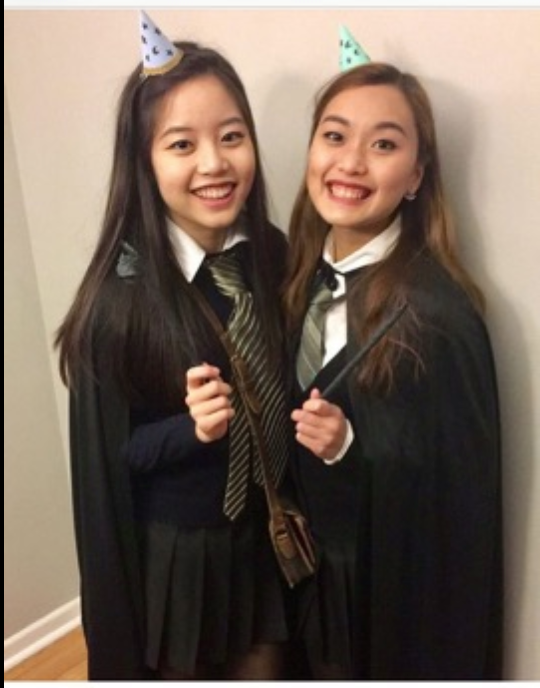
\includegraphics[width=0.5\textwidth]{wiz.png}
\end{figure}
\begin{figure}
\centering
\caption{Sushi. The person on the right is a sushi chef. Allegedly.}
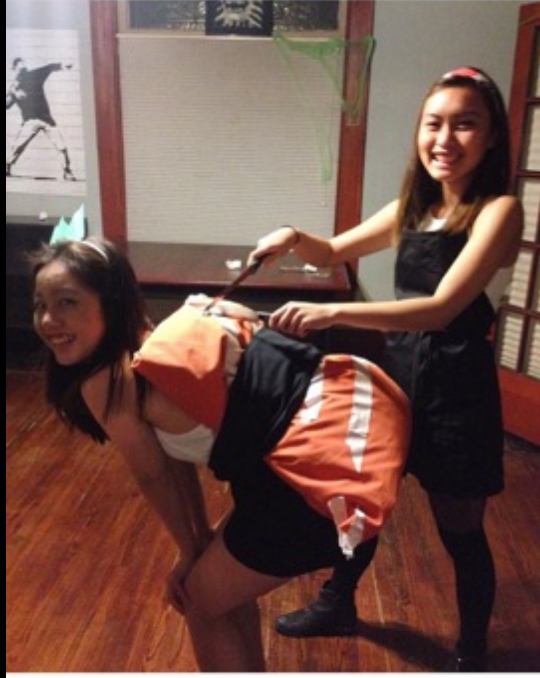
\includegraphics[width=0.5\textwidth]{sus.png}
\end{figure}
\begin{figure}
\centering
\caption{Lack of preparedness can be defended with an elaborate explanation. This is a ghost. Or a nun.}
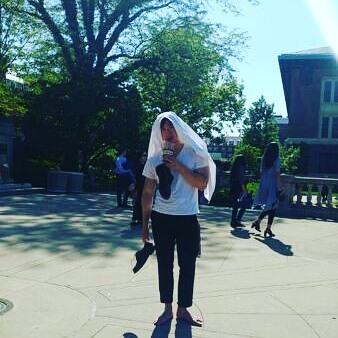
\includegraphics[width=0.5\textwidth]{ghost.jpg}
\end{figure}
\end{document}






